\documentclass[a4paper]{ctexart}
\usepackage{geometry}
\usepackage{pstricks}
\usepackage{multicol}
\usepackage{pst-plot}
\usepackage{graphicx}
\usepackage[]{url}
\geometry{left=2cm,right=2cm,top=2.5cm,bottom=2.5cm}
\usepackage{graphicx}
\newcommand{\HRule}{\rule{\linewidth}{0.5mm}}

\author{严春伟\\
    互联网研发中心\\
    1201213679
\and 王永庆\\
    嵌入式实验室\\
    xxxx
}

\begin{document}
\begin{titlepage}
    \begin{center}
    \textsc{\LARGE X509加密社交系统实现}\\[1.5cm]
    \textsc{\Large 密码学大作业}\\[4.5cm]
    % Title
    \HRule \\[0.4cm]
    
\includegraphics[width=0.55\textwidth]{./logo}\\
    \HRule \\[2.5cm]
% Author and supervisor
    \begin{minipage}{0.4\textwidth}
        \begin{flushleft} \large
            \begin{center}
            严春伟\\
            1201213679\\
            互联网研发中心
            \end{center}
        \end{flushleft}
    \end{minipage}
    \begin{minipage}{0.4\textwidth}
        \begin{flushright} \large
            \begin{center}
                王永庆\\
                1201213674\\
                现代数字信号处理实验室
            \end{center}
        \end{flushright}
    \end{minipage}

    \vfill

    % Bottom of the page
    {\large \today}
    \end{center}
\end{titlepage}

\section{需求分析}
\par 在实际工作或者学习中,特别是在企业或者学校中,经常会有比较正式和重要的新闻和公告。 目前现成的接受工具包括电子邮箱、即时通信(IM)、社交网络(人人网、QQ等)。其中,就我学校环境来看,用的比较多的包括邮箱(企业邮箱,sz.pku.edu.cn),以及班级群。但是通知公告嫁接在常规的信息工具之上会有一些不方便,如图\ref{fig:school-mail}, 图\ref{fig:qq-message}.
    \par 图\ref{fig:school-mail} 是学校的公共邮箱,很多正式的通知公告会由相关的职能部门发给每一位学生,但是由于学生的身份并没有详细的划分,总会有很多信息公告甚至垃圾邮件被盲目推送给并不相关的学生。
    \par 比如图中汇丰商学院的讲座信息也发送给了我们信息工程学院的学生,相信大部分学生都不需要这样的信息.
    \par 图\ref{fig:qq-message}是我们班级群聊天记录一小部分的截图。
    \par 可以看到由于QQ群本身就是一个聊天交流的工具,并不完全能够胜任通知的要求,主要有两个原因:
    \begin{enumerate}
        \item 在老师发送通知之后,一些与之无关的聊天讨论仍会继续,这导致了正式的通知会很快淹没在无关的聊天刷屏中
        \item QQ本身只是一个聊天工具而已,并不能将之与学校及其他机构正式的公告平台等同,很多同学并不会每天上QQ,这降低了信息的传达效果。
    \end{enumerate}

    \begin{figure}
        \centering
        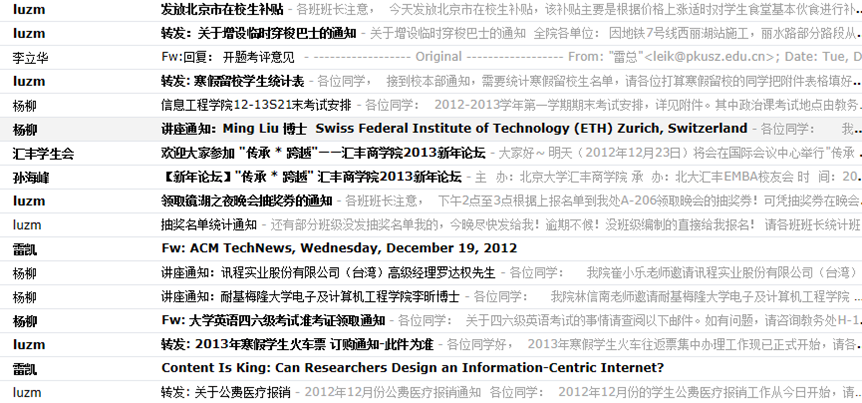
\includegraphics[width=500pt]{File8.png}
        \caption{\small \sl 学校内公共邮箱内的邮件比较杂乱.}
        \label{fig:school-mail}
    \end{figure}
    \begin{figure}
        \centering
        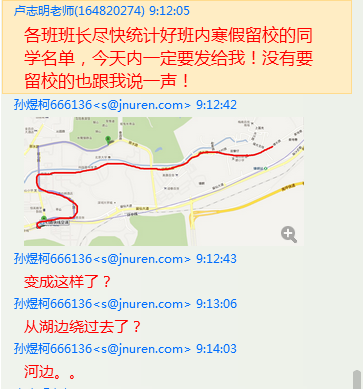
\includegraphics[width=300pt]{File2.png}
        \caption{\small \sl QQ中的公告信息很容易淹没在无关的讨论中.}
        \label{fig:qq-message}
    \end{figure}
    \par 考虑到这些,我们尝试去实现一个专业公共的平台。

\section{实现设想}
    \par 我们实现的核心思想是,实现一个平台,能够将日常所需要的通告信息聚集起来,对于我们学生,一般的信息包括学校学院最新的新闻,还有的就是通知公告.
    \par 我们实现了一个爬虫,能够自动爬取深圳研究社官网(\url{http://pkusz.edu.cn}),信息工程学院(\url{http://ece.pku.edu.cn})的首页新闻.
    \par 通过群组的概念将通知信息进行归类,用户可以添加或者退出群组来自由选择自己所需要的公告信息来源。 同时,我们有限度地支持回复讨论的功能,并很注重将回复与正式的通告的区分。信息以推送的方式发送给每一位用户,为了方便了解用户对信息的回馈,我们实现了一个统计的功能,可以让信息推送人很方便地统计对信息公告感兴趣的用户(比如,推送一个活动或讲座的公告后,会有哪些用户有意愿参加)。


\newpage
\section{实现及环境}
    \begin{center}
    \begin{tabular}[]{l|l}
        \hline
        开发语言        &   Python2.7       \\ 
        \hline
        网络框架        &   web.py          \\
        \hline
        数据库          &   sqlite          \\
        \hline
        爬虫框架            &   Scrapy          \\
        \hline
        数据库操作框架  &   sqlalchemy      \\
        \hline
        javascript 框架 &   jQuery          \\
        \hline
        X509实现        &   OpenSSL         \\
        \hline
        运行环境        &   Linux Mint 14   \\
        \hline
    \end{tabular}
    \end{center}

    \newpage
    \section{数据库设计}
    \begin{center}
        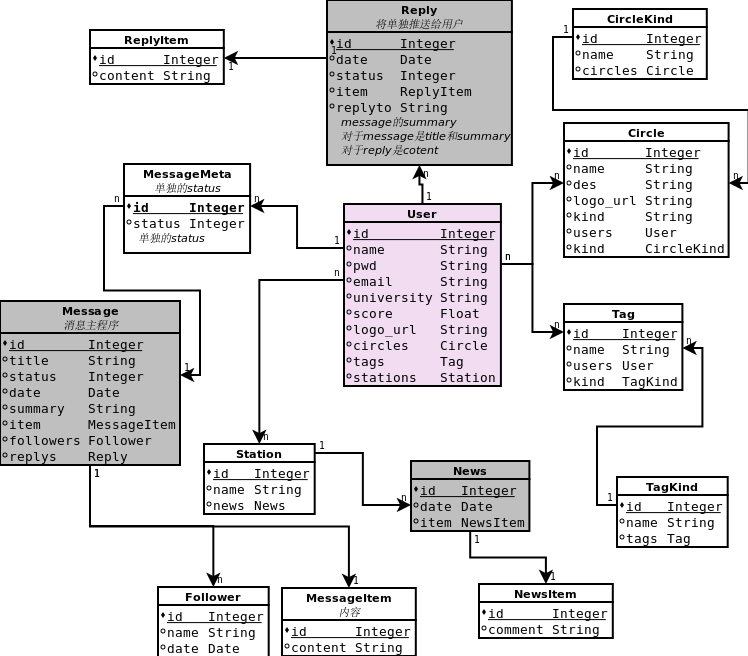
\includegraphics[width=500pt]{db.png}
    \end{center}

\section{X509协议}

\section{运行演示}
    \subsection{基本界面}
    \begin{figure}[htpb]
        \begin{center}
            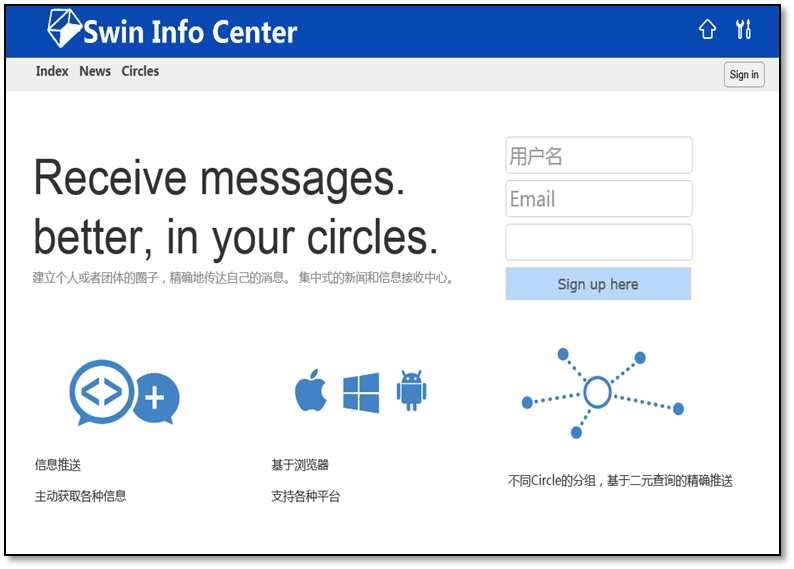
\includegraphics{File3.png}
            \caption{\small \sl 首页}
            \label{fig:website-index}
        \end{center}
    \end{figure}
    \begin{figure}[htpb]
        \centering
        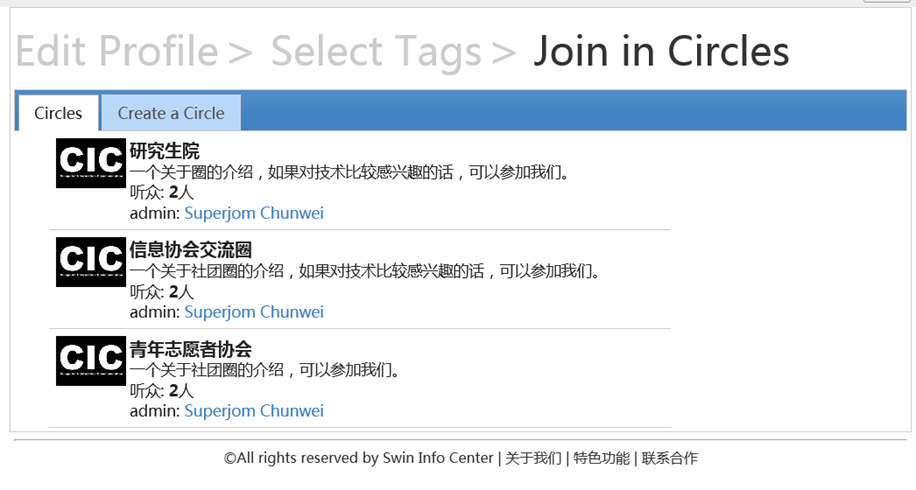
\includegraphics{File4.png}
        \caption{\small \sl 群组}
        \label{fig:website-circle}
    \end{figure}
    \begin{figure}[htpb]
        \centering
        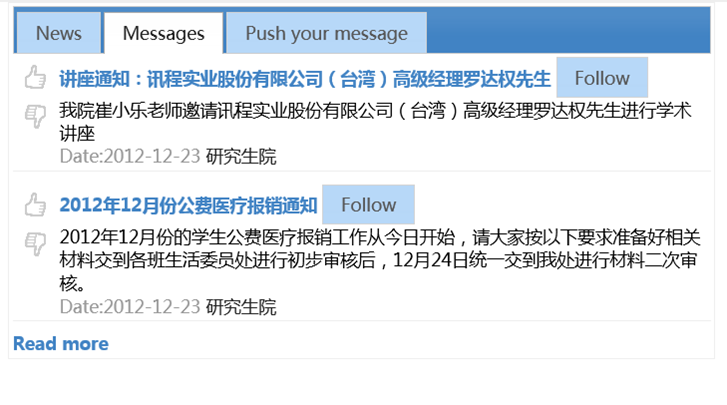
\includegraphics{File5.png}
        \caption{\small \sl 推送的信息}
        \label{fig:pushed-message}
    \end{figure}
    \begin{figure}[htpb]
        \centering
        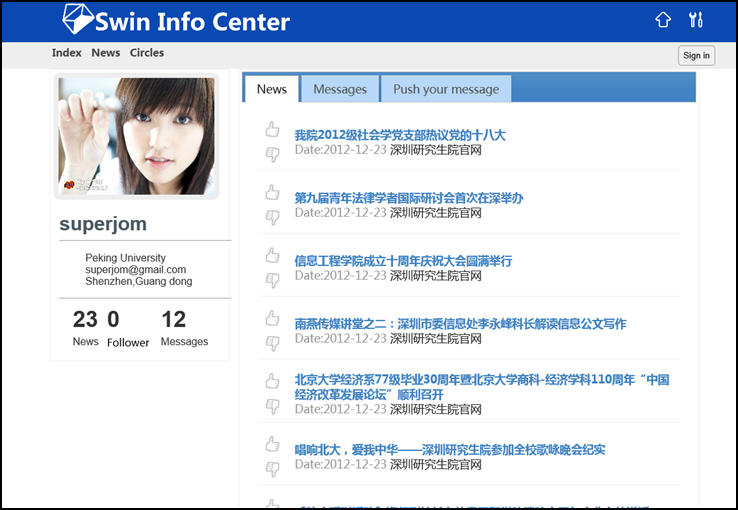
\includegraphics{File6.png}
        \caption{\small \sl 爬取的新闻}
        \label{fig:website-news}
    \end{figure}

    \subsection{\small \sl 功能演示}
    \begin{figure}[]
        \centering
        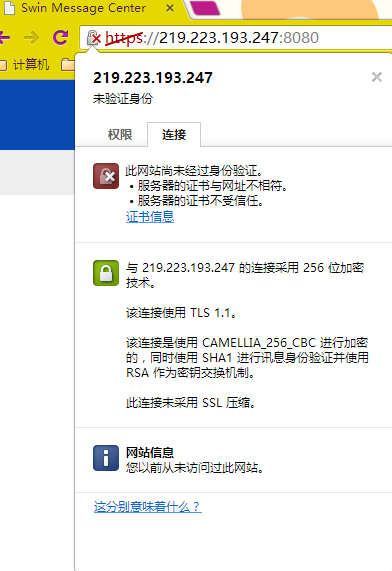
\includegraphics{zhengshu1.png}
        \caption{\small \sl 用Google 浏览器https浏览本平台}
        \label{fig:website-zhenshu1}
    \end{figure}
    \begin{figure}[]
        \centering
        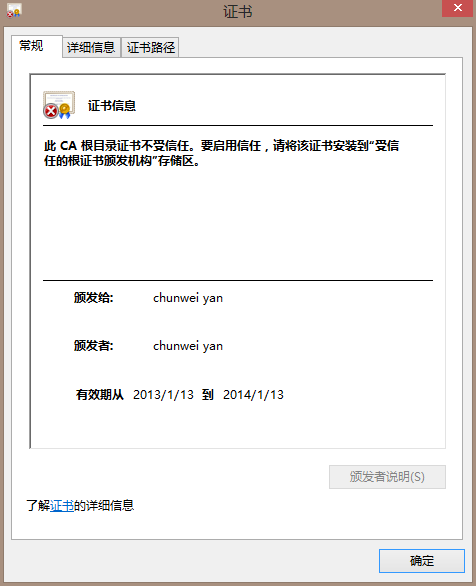
\includegraphics{zhengshu2.png}
        \caption{\small \sl 具体证书}
        \label{fig:zhengshu2}
    \end{figure}

    \begin{figure}[]
        \centering
        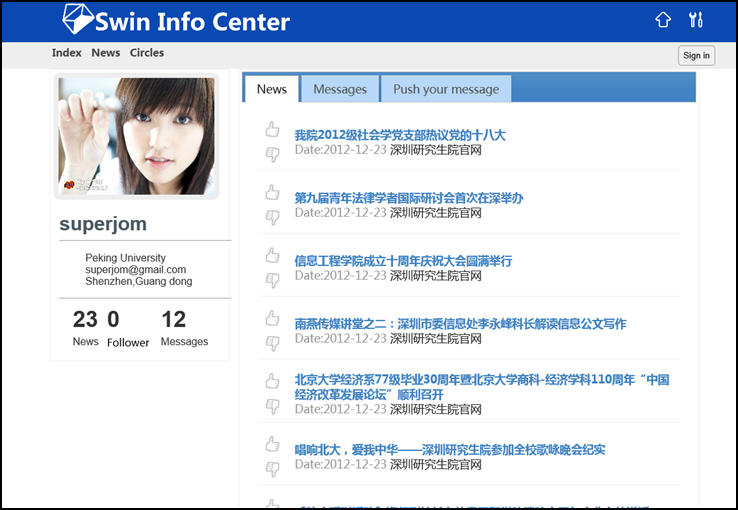
\includegraphics{File6.png}
        \caption{\small \sl 新闻列表}
        \label{fig:news-list}
    \end{figure}
    \par 图\ref{fig:news-list}表示的是我们从深圳研究生院网站以及信息工程学院网站抓取的最新的新闻。
    \begin{figure}[]
        \centering
        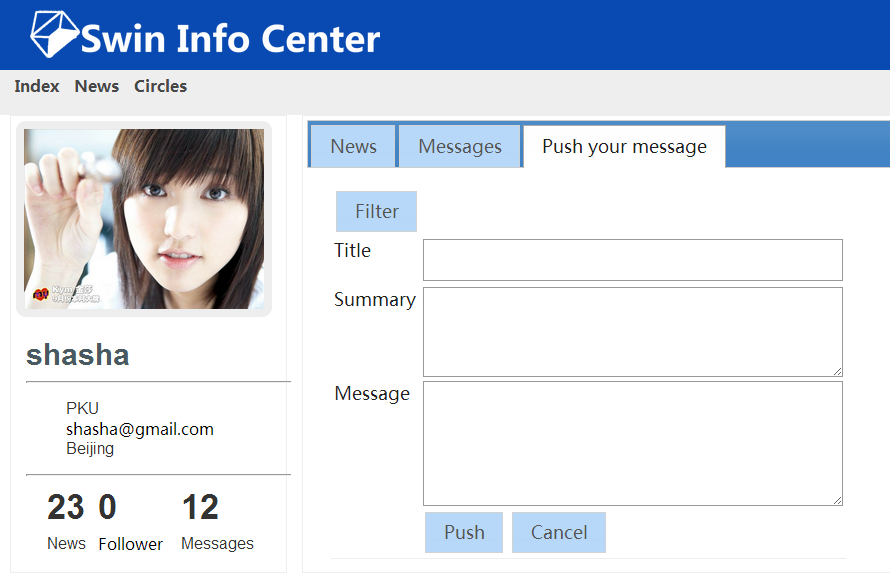
\includegraphics[width=400pt]{message.png}
        \caption{\small \sl 信息推送}
        \label{fig:push-message}
    \end{figure}
    \begin{figure}[]
        \centering
        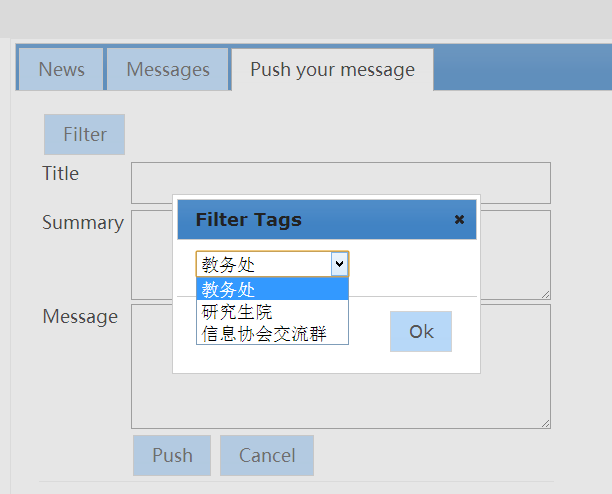
\includegraphics[width=300pt]{filter.png}
        \caption{\small \sl 推送群组选择}
        \label{fig:filter-circle}
    \end{figure}
    \par 图\ref{fig:filter-circle}表示,我们实现了一个类似QQ群组的功能,不同的信息公告通过群组进行分类,筛选。用户选择了一个群组就相当于接受这个群组的信息公告。 公告只能由该群组的拥有者推送出去,给每一位听众,听众的回馈会直接传达给管理者,但是不会被推送给其他用户。
    \begin{figure}[]
        \centering
        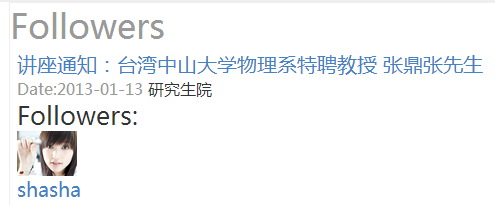
\includegraphics[width=300pt]{followers.png}
        \caption{\small \sl 统计参加用户}
        \label{fig:follow-message}
    \end{figure}
    \par 图\ref{fig:follow-message}展示的是用户统计功能,通过图\ref{fig:pushed-message}中的Follow按钮,用户可以对信息进行相关的回馈,比如讲座或者活动,点选follow按钮表示是要参加,信息的拥有者可以在自己的后台很方便地看到所有Follow的用户的列表,便于统计人数。
    



\end{document}

